% Need to review Justin Grimmer

\chapter{Computational Social Science}
\label{ch:css}

While the previous chapters were mostly retrospective analyses,
computational social science is mostly in the ``here and now''.  The
role of text analysis is to provide evidence for how people relate to
each other and to their environment in particular contexts, for
example social, political, or economic interactions.  The specific
expression of any particular document is usually of less importance.
As a result, social science focuses on data being generated in the
most recent hours, days, or weeks to inform intelligence analysts, brand
monitors, journalists, or social scientists.  The underlying problem
is the same, however: these stakeholders are interested in what people
have to say but cannot read all of the data at their disposal.

\index{survey}
Historically, social science asks questions about opinions. What candidate is
preferred in a particular part of the country? Do people like a
new restaurant or product?  These questions are often answered by
polling: social scientists would head out into the world, gather a
statistically significant survey sample, and extrapolate to the
broader population.

These techniques remain foundational, but they take time.  A
company needs to know if it has an issue with a product immediately,
particularly if its good name is being dragged through the mud on
social media~\citep{bowen-16}.  However, the reason for the acute time
pressure can also be the solution: if a company is able to quickly see
that it has a social media problem, it can more quickly intervene and
correct the issue.

\index{influenza}
\index{approval rating}
Traditional social science methods are labor intensive, take a long
time, or are impossible for sensitive subjects.  For instance, surveys
of influenza take too long to be useful compared to the life cycle of
influenza's progression~\citep{broniatowsky-15}, and approval ratings
may be too slow in the run-up to an election~\citep{oconnor-10}.  Using
Twitter and Google searches results in more accurate information
faster.

\index{pollution in China}
Directly communicating with some
populations may be difficult.  Using social media presents an
alternative~\citep{wang:paul:dredze-15}, as individuals share
information more freely than official news agencies (which, for example, may suffer
from official censorship in the case of opinions about pollution in China) or in
school-administered surveys (which can suffer from self-censorship in
the case of sexuality or drug use).  Topic models and other large-data approaches
that can look at vast quantities of text help overcome some of the
obstacles to fast-response social science.

The observational nature of topic models is both a weakness and a
strength.  Analyzing documents through social media collection can
induce threats to validity. Researchers cannot necessarily control the
populations producing documents, the forum in which documents are
written, or the subject of documents.  At the same time, observational
models have the advantage of increased potential for discovery.  In a
survey, researchers have to specify every question that will be asked.
That control is good for ensuring validity, but risks missing whole
categories of opinion that might not be obvious to researchers.  Topic
models can complement this type of carefully designed survey by
unearthing issues or factors important to participants
whether or not those issues were anticipated.  Thus unsupervised
models can help in identifying questions that researchers ``forgot to
ask''.

\paragraph{Prediction and Interpretation}

\index{prediction vs. interpretation}
A common theme in using topic models is whether models
should prioritize \emph{prediction} or \emph{interpretation}. 
Different topic models privilege each of  these approaches.
The distinction between model applications mirrors, to some extent,  the distinction between quantitative and qualitative social science.
Predictive applications are closer to quantitative methodologies that focus on regression-based methods that have clear input and output variables.
Interpretative applications are closer to qualitative methodologies that use human intuition to explain complex processes.
At the same time, the use of topic models blurs the boundary between these two methodologies.
Even when used to support qualitative work, topic models apply computation, and insulate researchers to an extent from pre-conceived biases (although they bring their own modeling assumptions).
Similarly, even when used to support quantitative work, topic models enable researchers to establish quantitative relationships between document metadata variables and variables derived from messy, unstructured text that might otherwise not have supported  quantitative analysis.

The previous chapters have focused on interpretation: can a user
understand the output of a model?  But for supervised models, there is
a question of how well the model can predict some parameter of interest, such as sentiment or user engagement.  

To some extent, these are not always in conflict.  \citet{ramage-10b}
show that topic model features can improve tweet categorization, as
do \citet{blei-07b} for supervised \abr{lda}.  However, changing the
objective function can further improve predictions~\citep{zhu-09}.

\index{interpretability}
However, sometimes improved interpretability
(Chapter~\ref{sec:coherence}) hampers the ability of the model to
predict content.  This is true of both words within a document and
document labels.  \citet{chang-09b} showed that complicated topic
models do a better job of predicting held-out documents but make less
sense to a user.  \citet{Nguyen-15:anchor} show that supervised models
offer better predictions with additional topics but the topics are
less interpretable.

\section{Topic Models for Qualitative Analysis}

\index{Facebook}
A common task in qualitative social science is to develop high-level theories that explain social processes based on low-level observations, such as field reports or ethnographic notes.
One way to operationalize this process is the grounded theory method~\citep{glaser-67}.
Grounded theory describes a process for iteratively developing theories through repeated reading of source material.
\citet{baumer-17} compare a manual grounded theory analysis and a topic model-based analysis of survey response text describing people's experiences attempting to voluntarily leave Facebook.

\index{grounded theory}
They find that there are both theoretical and empirical connections between these two approaches.
At the theoretical level, both grounded theory and probabilistic topic model algorithms are iterative, beginning with rough, low-quality models/theories and refining them through repeated passes through the documents.
Both methods also seek to maintain a close connection between the abstract representation and the original data set: in Gibbs sampling, topics are ``grounded'' in specific word tokens.
At the empirical level, \citet{baumer-17} find close connections between the themes discovered by researchers manually applying grounded theory procedures and topics discovered by an \abr{lda} model.
But this result should not imply that human analysis is of no additional value.
They report that the thematic meaning of \abr{lda} topics was not immediately apparent from simple lists of high-frequency words.
Rather, the model was most useful as a way of suggesting a topic-specific ``reading list.''
The ``meaning'' of topics was only clear at the theory level by browsing the documents that had unusually high representation of that topic.
As such the topic model can best be thought of as a tool for applying grounded theory more efficiently and with greater insulation from human biases. 

\section{Sentiment Analysis}

\index{sentiment analysis}
A useful way to think of the application of topic models in quantitative social science is as a means of deriving a numeric variable from text.
Specific topics in a document can stand in for themes that may not be otherwise easily measurable.
These inferred topic variables can then be added to standard statistical methods to find connections between topics and non-textual variables.
As a motivating example, we first consider sentiment analysis~\citep{pang-08}.  Here, the goal is to determine the
``sentiment''---e.g., positive or negative opinions---associated with
a piece of text.  For example, ``Chipotle is great!'' would be
associated with positive sentiment, while ``Chipotle made me sick''
would be associated with negative sentiment.

While commercial applications of sentiment analysis are mostly for
identifying whether people like a product or company, there are wider
social science applications of examining large corpora to determine
authors' \emph{internal state}.  For example, political scientists may
want to classify social media users as liberal or conservative based on their online
commentary.

Topic models can help these tasks by dividing a problem into topics.
The contextual disambiguation provided by topics can be useful in 
narrowing the range of applicable subjects.
For example, ``Apple'' can appear in tech news as well as a food
ingredient; someone monitoring the seller of iPods and iPhones would
not want to be confused by social media commentary complaining about 
the low quality of a Red Delicious. 
Contextual disambiguation can also be useful because the implied sentiment of words 
can vary considerably between domains.
The term ``surprising'' could be positive in a book review, but 
strongly negative in an automobile review.

Topic-based sentiment analysis can, however, be problematic.
The objective of a topic model is to identify and separate the latent factors that best explain the way combinations of words appear together in documents.
Sentiment can be subtle, and may not present the strongest signal to an algorithm.
For example, even though restaurant reviews are specifically intended to be sentiment-bearing, topic models trained on restaurant reviews mostly align with {\em types} of restaurants, producing topics representing cuisines, such as Chinese, Mexican, and Thai.
Topic models also lose their value if you want to \emph{contrast}
sentiment within a topic.  While a topic model can find people
discussing Chipotle burritos online, it cannot separate the lovers from
haters.  Thus, \emph{distinguishing} topics based on their sentiment
can help a user better understand how topics and sentiment interact in
a dataset.  This requires modifying the topic model to make it aware
of the underlying sentiment.

% Sentiment is an example of metadata, which can be visualized to
% better understand a corpus (see viz).

\section{Upstream and Downstream Models}

To distinguish topics based on their sentiment, the model must be
aware of a non-textual variable that represents sentiment.
In the language of probabilistic models,
sentiment and topic are modeled \emph{jointly}.  That is, there is for each document a
probability distribution over both the sentiment variable $y$ and
the topic assignments $z$.

\index{upstream vs. downstream models}
There are two general kinds of joint models that incorporate metadata
such as sentiment: upstream and downstream models.  The distinction is
based on the generative story of topic models (Chapter~\ref{ch:intro}): is
sentiment before (upstream) or after (downstream) topics in the
generative story?

% Put in graphical model examples of upstream and downstream models

Upstream models assume that external variables such as sentiment come first in the generative
story.  That is, there will be different topics given the underlying
sentiment.  This can come in the form a hard-coded distribution~\citep{mei-07b}, a prior learned from observed
sentiment~\citep{mimno-08}, or from a latent variable that can serve as
a proxy for sentiment~\citep{lin-09}.  Upstream models are often
easier to implement and are more flexible~\citep{stewart-14} because they do not need to specify a generative distribution that matches the form of the variable.

\index{Gaussian distribution}
In contrast, downstream models explicitly predict variables such as sentiment
\emph{given} text.  If the goal is to later predict sentiment given
raw text with the help of topic models, downstream models can work
better than upstream models.  These models are often called
``supervised'' topic models after supervised
\abr{lda}~\citep[\abr{slda}]{blei-07b}, which use a document's topics to predict
the downstream sentiment using regression: a document's sentiment~$y_d$ is
assumed to come from a Gaussian distribution with mean $\eta^\top \bar
z$, where $\bar z$ is a normalized vector of all of the topics that a
document uses and $\eta$ is a regression parameter that describes the
sentiment of each topic.

\index{supervised latent Dirichlet allocation}
During inference, the words and sentiments work together to find
combinations of topic and sentiment that make sense.  While
``vanilla'' topic models seek to find clusters of words that make
sense together, if a topic is associated with documents that have many
different sentiment values, it will have to learn a less focused distribution over
sentiment scores, resulting in lower probability.  

\begin{figure}
  \begin{center}
    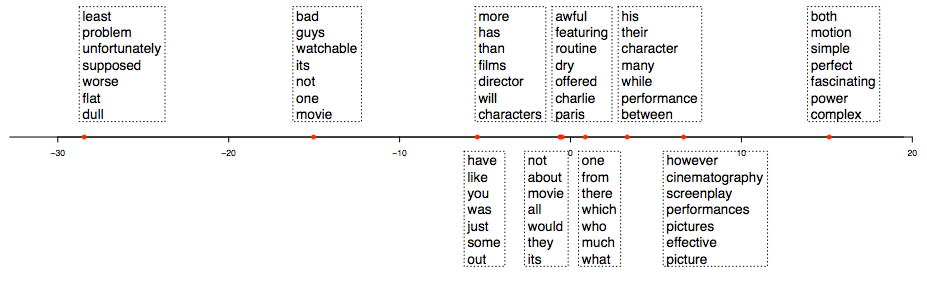
\includegraphics[width=1.0\linewidth]{figures/slda}
  \end{center}
  \caption{Example topics learned by supervised \abr{lda} from
    \citet{blei-07b}.  Each topic is not just a collection of words
    but also has a regression score~$\eta$ that explains whether it is
    associated with positive sentiment (right) or negative sentiment
    (left).}
  \label{fig:slda-topics}
\end{figure}

Consider Figure~\ref{fig:slda-topics}.  If a topic has an inconsistent
sentiment value (for example, a negative sentiment document in a
positive sentiment topic), inference will try to move the negative
sentiment documents to topics with consistent sentiment~$\eta$ {\bf
  and} consistent words.  

These models form the foundation for the models and problems we
discuss in the rest of this section.

\section{Understanding Stance and Polarization}

Another form of internal state is \emph{stance}: which side does a
person take on an issue.  This can take many forms: are you for or
against a proposal, are you a Democrat or a Republican, or are you a
fan of the original Star Trek or the new version?

\index{aspect model}
Upstream models can discover these sides by incorporating stance into
the generative model.  For example, several authors---\citet{zhai-04},
\citet{lu-08}, and \citet{paul-10}---develop topic models that allow readers to compare
aspects of a topic.  They posit that each comparative
``side'' has a distribution over words that it uses generally
\emph{and} that each side had its own take on how it discusses a
topic.  Within a document, each word is chosen either from a side's
background distribution, a side's version of the topic, or from the
topic's ``neutral'' words.  For instance, Israelis and Palestinians
both use ``attacks'', ``civilians'', and ``military'' in discussing
unrest in Israeli-occupied Palestine, but the Israeli side uses
``terrorist'' and ``incitement'', while the Palestinian side focuses
on ``resistance'' and ``occupation''.

The interaction between sentiment and aspect is unclear.  Some
aspects are independent of sentiment, and other aspects are
particularly charged.  \citet{jo-11} develop a model that first draws
sentiment distributions that constrain the aspects discussed in a
document.


\begin{figure}[t]
\begin{center}
    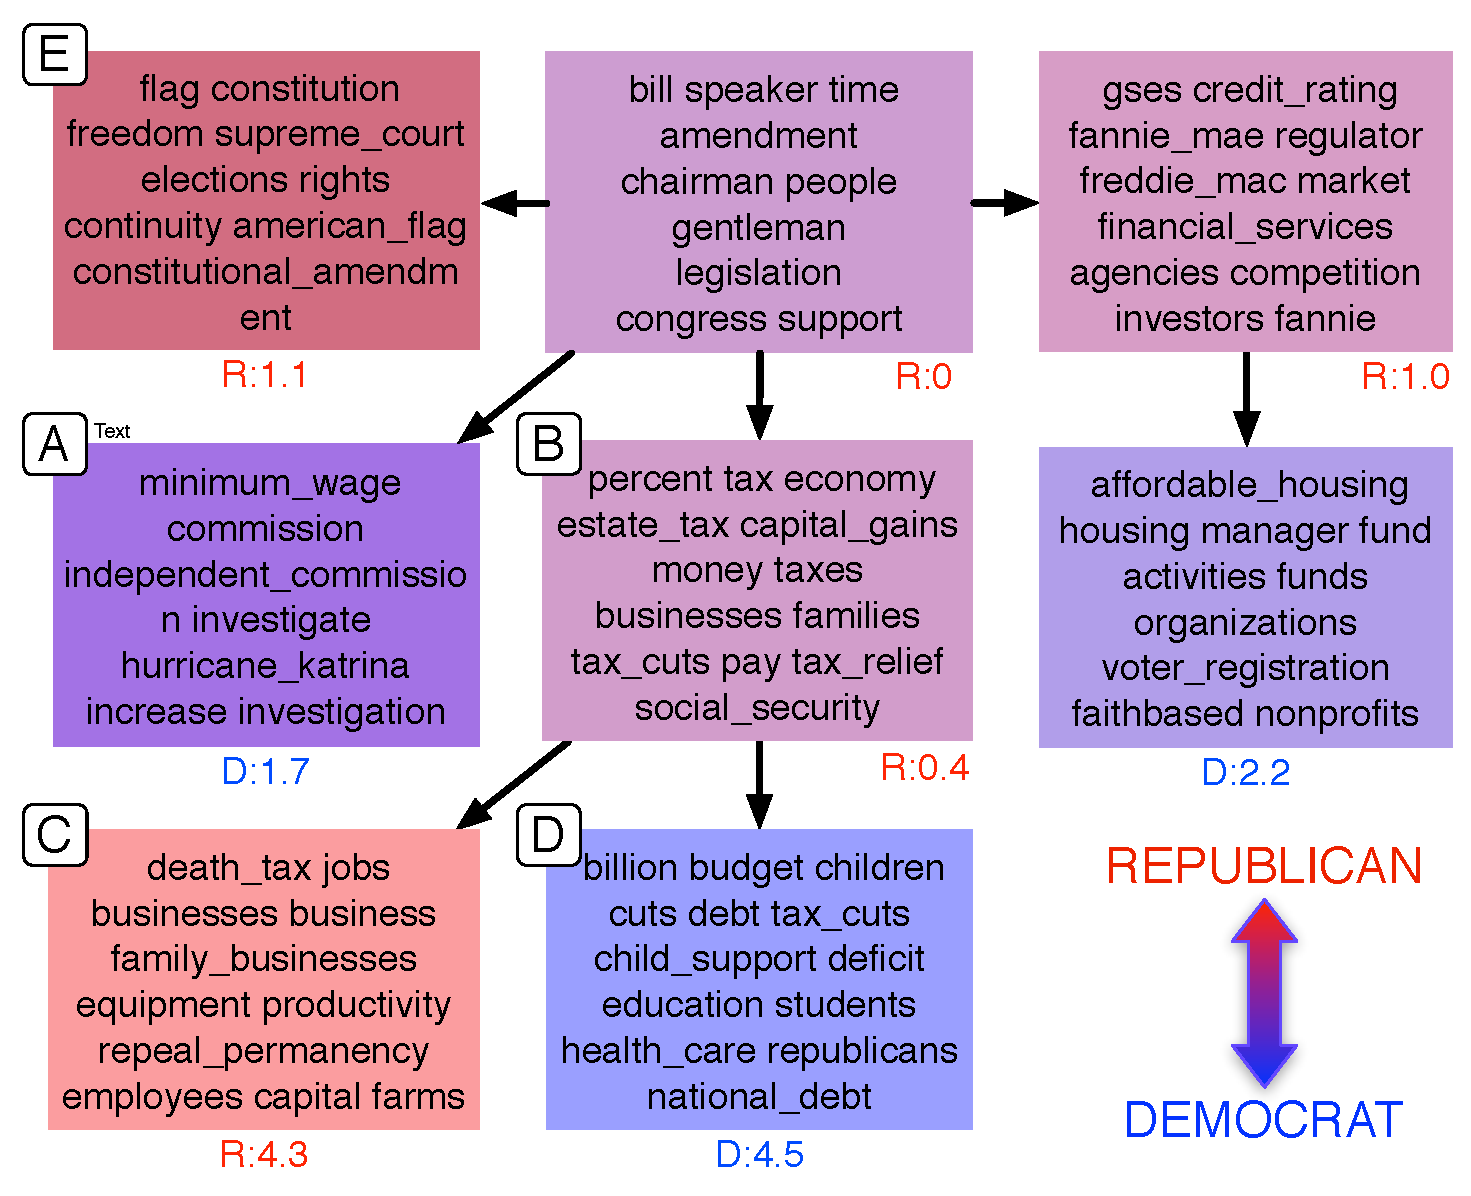
\includegraphics[width=0.65\textwidth]{figures/ideology_topics_vert}
\end{center}
    \caption{
       \small Topics discovered from Congressional floor debates using
       a downstream model to capture speaker's ideology.  Many
    first-level topics are bipartisan (purple), while lower level topics are
    associated with specific ideologies (Democrats blue, Republicans red). For example,
    	the ``tax'' topic (B) is bipartisan, but its Democratic-leaning child (D) focuses on
    	social goals supported by taxes (``children'', ``education'', ``health care''), while
    	its Republican-leaning child (C) focuses on business implications (``death tax'', ``jobs'',
    	``businesses'').  The number below each
    topic denotes the magnitude of a learned regression parameter associated
    with that topic.  Colors and the numbers beneath each topic show the
    regression parameter $\eta$ associated with the topic.  From \citet{nguyen-13:shlda}.
    } \label{fig:shlda-taxes}
\end{figure}

Downstream models can also capture these divisions as well.
\citet{nguyen-13:shlda} predict whether a speaker is Republican or
Democrat\footnote{In downstream models, which variables to use in the
  prediction is often up for debate.  Using lexical
  terms~\citep{titov-08,zhao-10} in a log-linear model typically works
  better: it is able to capture word-specific nuances of sentiment and
  model situational sentiment (e.g., ``unpredictable'' is good for a
  book but bad for a car's steering).  However, it leads to a more
  complicated, less interpretable model.} based on the versions of
topics they discuss, extending the non-predictive model of
\citet{grimmer-09}.  For example, Republicans are more likely to
discuss taxes than Democrats, but Democrats focus on the
good that comes out of taxes (Figure~\ref{fig:shlda-taxes}).

% Need to cite Grimmer

\index{nested Dirichlet process}
However, there are not always two sides to an issue.  A probabilistic
solution to this model is the nested Dirichlet
process~\citep{blei-07}.  These hierarchies induce a non parametric
hierarchy over an unbounded number of topics.  This corresponds to
agenda setting from political
science~\citep{Nguyen:Boyd-Graber:Resnik:Miler-2015}.


% Eisenstein

\section{Social Networks and Media}

We have talked about metadata that are independent for each user.
Sometimes, however, we are interested in metadata that describe the
relationships \emph{between} documents: which users follow each other
on Twitter, which scientific papers cite each other, or which webpages
link to each other.  This makes modeling more difficult, but we still
see the same division between upstream and downstream models: upstream
models assume that the communities form before we see words, while
downstream models use the words to explain which links we see.

\index{stochastic block model}
\index{mixed-membership block model}
The stochastic block model~\citep{holland-83} and its mixed-membership
descendant~\citep{airoldi-08} are prototypes for upstream models.
They posits that there are intrinsic groups of documents and links are
more likely inside the group than outside the group.  These groups are
analogous to the topics in topic models, except that the links are
``shared'' between documents.

However, the first probabilistic models of network structure ignored
the words in documents.  Because the network structure is tied to
author identity, it is natural to combine author identity with
an upstream model~\citet{mccallum-07,liu-09}, conditioning topics on
authors and the communities the authors belong to.

\index{link latent Dirichlet allocation}
Link \abr{lda} is the exemplar for downstream
models~\citep{nallapati-08} and include the text in the documents.  It
uses a regression on the topic allocations ($\theta$) rather than
topic assignments ($z$), in contrast to supervised \abr{lda} above.  Similarly, \citet{cha-12} use
followed users to model downstream documents.

Conditioning on the topic assignments can improve the algorithm's
ability to predict links on held-out documents,
however~\citep{chang-09a}.  This is because a regression based on the
allocations alone can use topics to explain links that aren't in the
document.  For example, if the model thinks there's a link between
documents because they both use Topic~14 but no words in the document
are assigned ($z_n=14$), then the model is unable to recreate this
prediction in a held-out document.  

Not all topic models applied to social network attempt to predict
links.  \citet{weng-10} use the network structure of Twitter to find
who is influential within a topic, and several models use links to
constrain documents that are linked together to be
similar~\citep{mei-08,sun-09,daume-09}.

In addition to explicit links in social networks, social media is also
shaped by implicit links between people in similar contexts---events,
cultural, or regional patterns that affect how people talk and what
they talk about.  \citet{mei-06} capture how topics vary across region
and time (e.g., when a hurricane strikes a region, those closest to
the eye of the storm will talk about it with greater volume and more
specifically).  Later work builds models location and topic
jointly~\citep{yin-11}.

In constrast, \citet{eisenstein-17} focuses on lexical variation,
capturing how social media neologisms like ``af'' (a post-position
intensifier, particularly of adjectives: e.g., ``the description was
evasive af'') spread from twin epicenters in southern California and
Atlanta to the whole of the US.

\subsection{Peculiarities of Social Media}
\label{sec:twitter-strange}

\index{Twitter}
\citet{hong-10} discuss how the short documents of social media
platforms like Twitter can confuse topic modeling algorithms, and
\citet{zhao-11} expand on the analysis, showing topical differences
(e.g., Twitter often briefly follows fleeting topics passionately).
Because a document is limited to 140 character, the admixture
assumptions of topic models are limited.  To capture trends over time
or across users, algorithms must also know connections between users
or group messages together over time~\citep{mehrotra-13}.  Other
researchers develop models with specific sparsity
properties~\citep{lin-14} to accomodate the peculiarities of Twitter.

\section{Summary}
\label{sec:css-summary}

Computational social science can unlock the emotion and hidden
factions often present in online discussions.  This is useful for
companies trying to understand their customers, for politicians trying
to target voters, for first responders reacting to a
disaster~\citep{kireyev-09}, and for academics trying to understand
how online communication morphs social norms.

However, as social networks increasingly span the entire globe,
assuming that a topic model is only in a single language is often a
poor assumption.  Indeed, even within a single country, topic models
can discover regional variation~\citep{eisenstein-10}.  In the next
chapter, we discuss how to cope with multilingual datasets and still
discover coherent, language-independent topics.


